\documentclass[1p]{elsarticle_modified}
%\bibliographystyle{elsarticle-num}

%\usepackage[colorlinks]{hyperref}
%\usepackage{abbrmath_seonhwa} %\Abb, \Ascr, \Acal ,\Abf, \Afrak
\usepackage{amsfonts}
\usepackage{amssymb}
\usepackage{amsmath}
\usepackage{amsthm}
\usepackage{scalefnt}
\usepackage{amsbsy}
\usepackage{kotex}
\usepackage{caption}
\usepackage{subfig}
\usepackage{color}
\usepackage{graphicx}
\usepackage{xcolor} %% white, black, red, green, blue, cyan, magenta, yellow
\usepackage{float}
\usepackage{setspace}
\usepackage{hyperref}

\usepackage{tikz}
\usetikzlibrary{arrows}

\usepackage{multirow}
\usepackage{array} % fixed length table
\usepackage{hhline}

%%%%%%%%%%%%%%%%%%%%%
\makeatletter
\renewcommand*\env@matrix[1][\arraystretch]{%
	\edef\arraystretch{#1}%
	\hskip -\arraycolsep
	\let\@ifnextchar\new@ifnextchar
	\array{*\c@MaxMatrixCols c}}
\makeatother %https://tex.stackexchange.com/questions/14071/how-can-i-increase-the-line-spacing-in-a-matrix
%%%%%%%%%%%%%%%

\usepackage[normalem]{ulem}

\newcommand{\msout}[1]{\ifmmode\text{\sout{\ensuremath{#1}}}\else\sout{#1}\fi}
%SOURCE: \msout is \stkout macro in https://tex.stackexchange.com/questions/20609/strikeout-in-math-mode

\newcommand{\cancel}[1]{
	\ifmmode
	{\color{red}\msout{#1}}
	\else
	{\color{red}\sout{#1}}
	\fi
}

\newcommand{\add}[1]{
	{\color{blue}\uwave{#1}}
}

\newcommand{\replace}[2]{
	\ifmmode
	{\color{red}\msout{#1}}{\color{blue}\uwave{#2}}
	\else
	{\color{red}\sout{#1}}{\color{blue}\uwave{#2}}
	\fi
}

\newcommand{\Sol}{\mathcal{S}} %segment
\newcommand{\D}{D} %diagram
\newcommand{\A}{\mathcal{A}} %arc


%%%%%%%%%%%%%%%%%%%%%%%%%%%%%5 test

\def\sl{\operatorname{\textup{SL}}(2,\Cbb)}
\def\psl{\operatorname{\textup{PSL}}(2,\Cbb)}
\def\quan{\mkern 1mu \triangleright \mkern 1mu}

\theoremstyle{definition}
\newtheorem{thm}{Theorem}[section]
\newtheorem{prop}[thm]{Proposition}
\newtheorem{lem}[thm]{Lemma}
\newtheorem{ques}[thm]{Question}
\newtheorem{cor}[thm]{Corollary}
\newtheorem{defn}[thm]{Definition}
\newtheorem{exam}[thm]{Example}
\newtheorem{rmk}[thm]{Remark}
\newtheorem{alg}[thm]{Algorithm}

\newcommand{\I}{\sqrt{-1}}
\begin{document}

%\begin{frontmatter}
%
%\title{Boundary parabolic representations of knots up to 8 crossings}
%
%%% Group authors per affiliation:
%\author{Yunhi Cho} 
%\address{Department of Mathematics, University of Seoul, Seoul, Korea}
%\ead{yhcho@uos.ac.kr}
%
%
%\author{Seonhwa Kim} %\fnref{s_kim}}
%\address{Center for Geometry and Physics, Institute for Basic Science, Pohang, 37673, Korea}
%\ead{ryeona17@ibs.re.kr}
%
%\author{Hyuk Kim}
%\address{Department of Mathematical Sciences, Seoul National University, Seoul 08826, Korea}
%\ead{hyukkim@snu.ac.kr}
%
%\author{Seokbeom Yoon}
%\address{Department of Mathematical Sciences, Seoul National University, Seoul, 08826,  Korea}
%\ead{sbyoon15@snu.ac.kr}
%
%\begin{abstract}
%We find all boundary parabolic representation of knots up to 8 crossings.
%
%\end{abstract}
%\begin{keyword}
%    \MSC[2010] 57M25 
%\end{keyword}
%
%\end{frontmatter}

%\linenumbers
%\tableofcontents
%
\newcommand\colored[1]{\textcolor{white}{\rule[-0.35ex]{0.8em}{1.4ex}}\kern-0.8em\color{red} #1}%
%\newcommand\colored[1]{\textcolor{white}{ #1}\kern-2.17ex	\textcolor{white}{ #1}\kern-1.81ex	\textcolor{white}{ #1}\kern-2.15ex\color{red}#1	}

{\Large $\underline{9_{28}~(K9a_{5})}$}

\setlength{\tabcolsep}{10pt}
\renewcommand{\arraystretch}{1.6}
\vspace{1cm}\begin{tabular}{m{100pt}>{\centering\arraybackslash}m{274pt}}
\multirow{5}{120pt}{
	\centering
	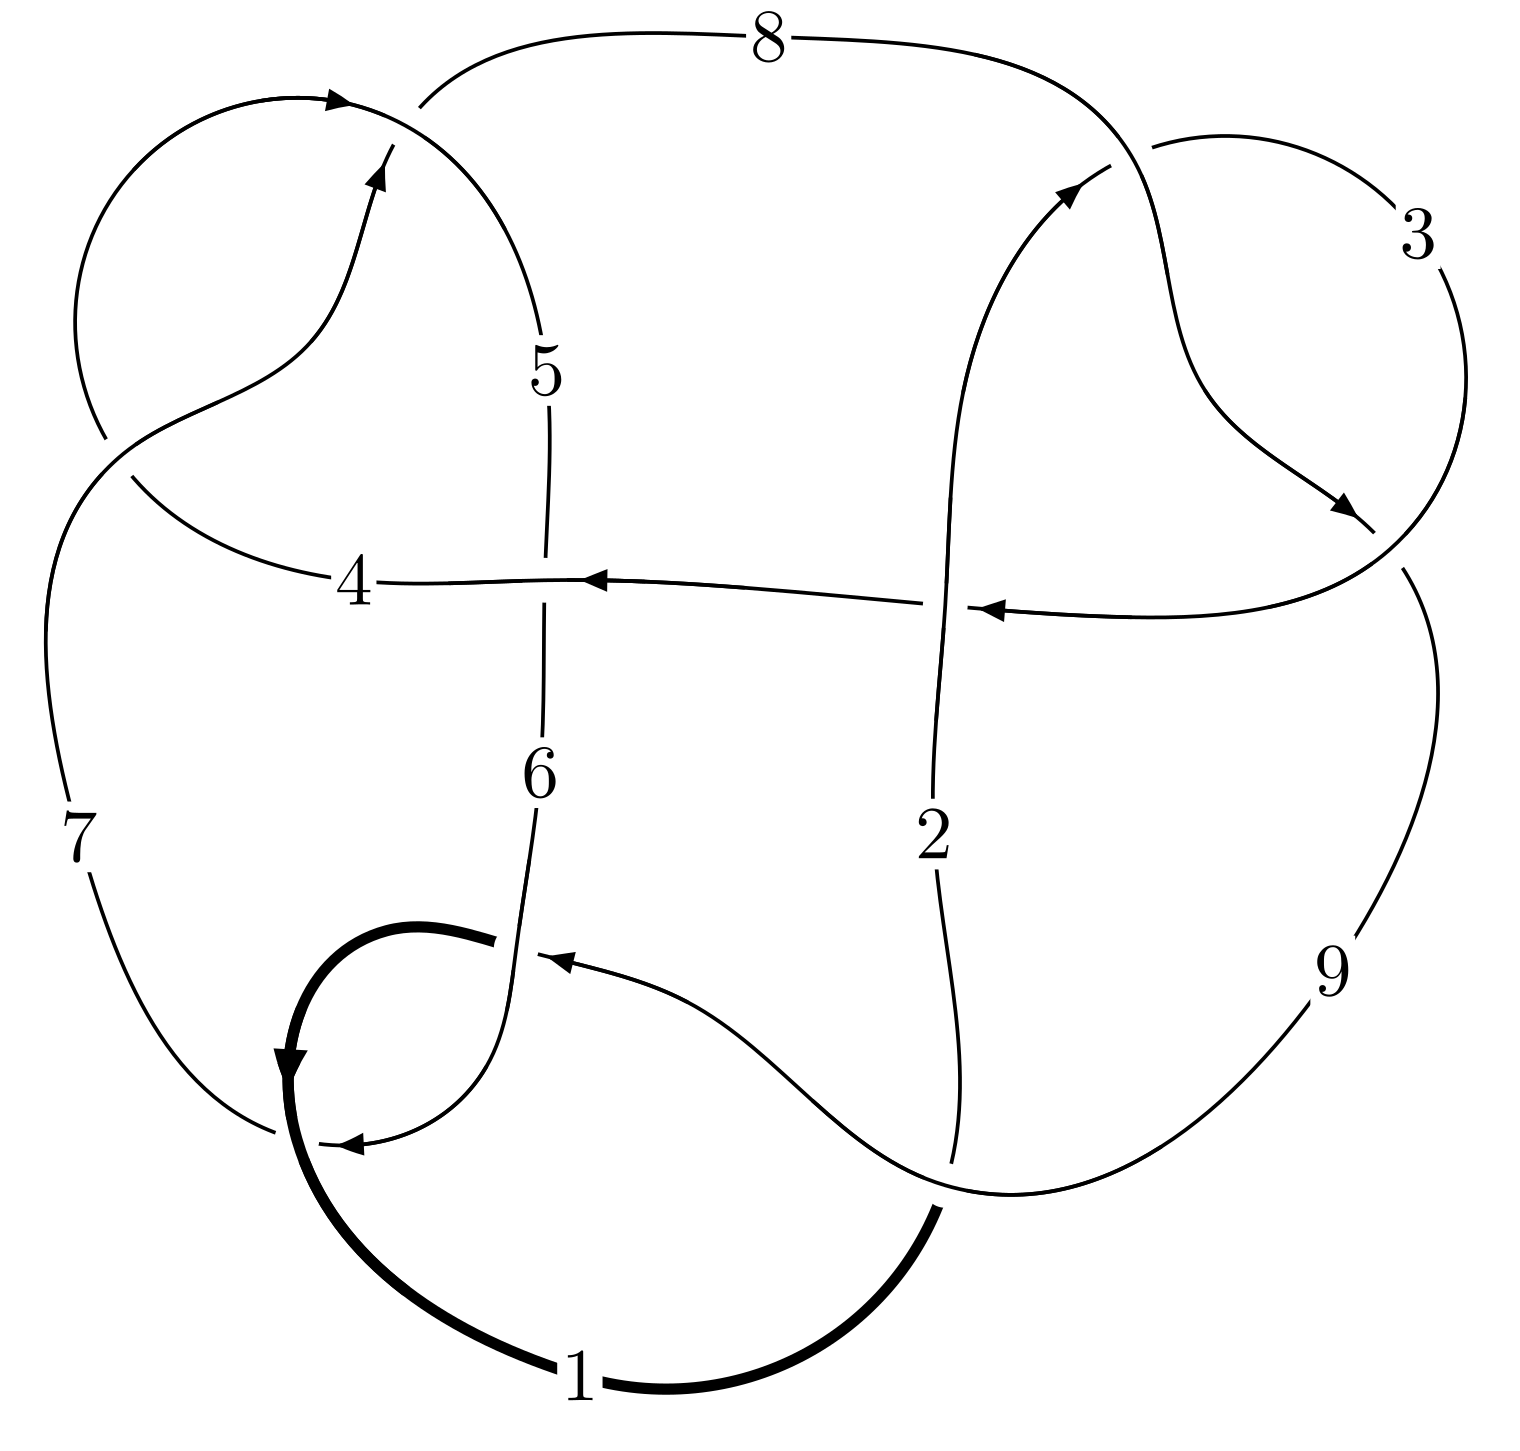
\includegraphics[width=112pt]{../../../GIT/diagram.site/Diagrams/png/63_9_28.png}\\
\ \ \ A knot diagram\footnotemark}&
\allowdisplaybreaks
\textbf{Linearized knot diagam} \\
\cline{2-2}
 &
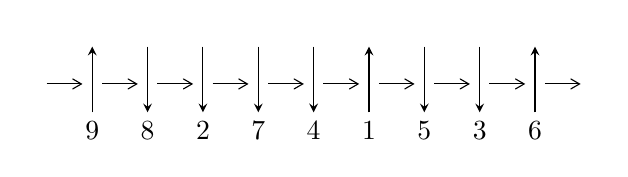
\begin{tikzpicture}[x=20pt, y=17pt]
	% nodes
	\node (C0) at (0, 0) {};
	\node (C1) at (1, 0) {};
	\node (C1U) at (1, +1) {};
	\node (C1D) at (1, -1) {9};

	\node (C2) at (2, 0) {};
	\node (C2U) at (2, +1) {};
	\node (C2D) at (2, -1) {8};

	\node (C3) at (3, 0) {};
	\node (C3U) at (3, +1) {};
	\node (C3D) at (3, -1) {2};

	\node (C4) at (4, 0) {};
	\node (C4U) at (4, +1) {};
	\node (C4D) at (4, -1) {7};

	\node (C5) at (5, 0) {};
	\node (C5U) at (5, +1) {};
	\node (C5D) at (5, -1) {4};

	\node (C6) at (6, 0) {};
	\node (C6U) at (6, +1) {};
	\node (C6D) at (6, -1) {1};

	\node (C7) at (7, 0) {};
	\node (C7U) at (7, +1) {};
	\node (C7D) at (7, -1) {5};

	\node (C8) at (8, 0) {};
	\node (C8U) at (8, +1) {};
	\node (C8D) at (8, -1) {3};

	\node (C9) at (9, 0) {};
	\node (C9U) at (9, +1) {};
	\node (C9D) at (9, -1) {6};
	\node (C10) at (10, 0) {};

	% arrows
	\draw[->,>={angle 60}]
	(C0) edge (C1) (C1) edge (C2) (C2) edge (C3) (C3) edge (C4) (C4) edge (C5) (C5) edge (C6) (C6) edge (C7) (C7) edge (C8) (C8) edge (C9) (C9) edge (C10) ;	\draw[->,>=stealth]
	(C1D) edge (C1U) (C2U) edge (C2D) (C3U) edge (C3D) (C4U) edge (C4D) (C5U) edge (C5D) (C6D) edge (C6U) (C7U) edge (C7D) (C8U) edge (C8D) (C9D) edge (C9U) ;
	\end{tikzpicture} \\
\hhline{~~} \\& 
\textbf{Solving Sequence} \\ \cline{2-2} 
 &
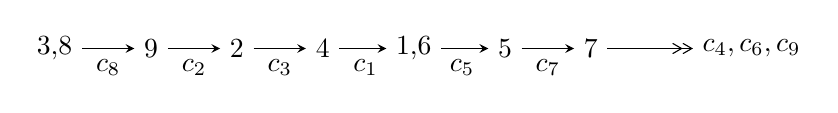
\begin{tikzpicture}[x=31pt, y=7pt]
	% node
	\node (A0) at (-1/8, 0) {3,8};
	\node (A1) at (1, 0) {9};
	\node (A2) at (2, 0) {2};
	\node (A3) at (3, 0) {4};
	\node (A4) at (65/16, 0) {1,6};
	\node (A5) at (41/8, 0) {5};
	\node (A6) at (49/8, 0) {7};
	\node (C1) at (1/2, -1) {$c_{8}$};
	\node (C2) at (3/2, -1) {$c_{2}$};
	\node (C3) at (5/2, -1) {$c_{3}$};
	\node (C4) at (7/2, -1) {$c_{1}$};
	\node (C5) at (37/8, -1) {$c_{5}$};
	\node (C6) at (45/8, -1) {$c_{7}$};
	\node (A7) at (8, 0) {$c_{4},c_{6},c_{9}$};

	% edge
	\draw[->,>=stealth]	
	(A0) edge (A1) (A1) edge (A2) (A2) edge (A3) (A3) edge (A4) (A4) edge (A5) (A5) edge (A6) ;
	\draw[->>,>={angle 60}]	
	(A6) edge (A7);
\end{tikzpicture} \\ 

\end{tabular} \\

\footnotetext{
The image of knot diagram is generated by the software ``\textbf{Draw programme}" developed by Andrew Bartholomew(\url{http://www.layer8.co.uk/maths/draw/index.htm\#Running-draw}), where we modified some parts for our purpose(\url{https://github.com/CATsTAILs/LinksPainter}).
}\phantom \\ \newline 
\centering \textbf{Ideals for irreducible components\footnotemark of $X_{\text{par}}$} 
 
\begin{align*}
I^u_{1}&=\langle 
u^3+b- u+1,\;-2 u^2+a- u+1,\;u^4+u^3- u^2- u+1\rangle \\
I^u_{2}&=\langle 
-2 u^{15}+8 u^{13}+3 u^{12}-14 u^{11}-10 u^{10}+8 u^9+14 u^8+6 u^7-6 u^6-11 u^5-3 u^4+3 u^3+2 u^2+b+u+2,\\
\phantom{I^u_{2}}&\phantom{= \langle  }-2 u^{15}+8 u^{13}+4 u^{12}-14 u^{11}-13 u^{10}+6 u^9+17 u^8+10 u^7-4 u^6-13 u^5-7 u^4+3 u^2+a+3 u+3,\\
\phantom{I^u_{2}}&\phantom{= \langle  }u^{16}+u^{15}-4 u^{14}-6 u^{13}+5 u^{12}+13 u^{11}+3 u^{10}-11 u^9-12 u^8-2 u^7+8 u^6+8 u^5+2 u^4-2 u^3-2 u^2-2 u-1\rangle \\
I^u_{3}&=\langle 
u^5- u^3+b+u,\;u^2+a,\;u^6- u^4- u^3+u^2+u+1\rangle \\
I^u_{4}&=\langle 
b+1,\;a+1,\;u-1\rangle \\
\\
\end{align*}
\raggedright * 4 irreducible components of $\dim_{\mathbb{C}}=0$, with total 27 representations.\\
\footnotetext{All coefficients of polynomials are rational numbers. But the coefficients are sometimes approximated in decimal forms when there is not enough margin.}
\newpage
\renewcommand{\arraystretch}{1}
\centering \section*{I. $I^u_{1}= \langle u^3+b- u+1,\;-2 u^2+a- u+1,\;u^4+u^3- u^2- u+1 \rangle$}
\flushleft \textbf{(i) Arc colorings}\\
\begin{tabular}{m{7pt} m{180pt} m{7pt} m{180pt} }
\flushright $a_{3}=$&$\begin{pmatrix}0\\u\end{pmatrix}$ \\
\flushright $a_{8}=$&$\begin{pmatrix}1\\0\end{pmatrix}$ \\
\flushright $a_{9}=$&$\begin{pmatrix}1\\u^2\end{pmatrix}$ \\
\flushright $a_{2}=$&$\begin{pmatrix}u\\u\end{pmatrix}$ \\
\flushright $a_{4}=$&$\begin{pmatrix}- u^3\\- u^3+u\end{pmatrix}$ \\
\flushright $a_{1}=$&$\begin{pmatrix}u^3\\u^3- u+1\end{pmatrix}$ \\
\flushright $a_{6}=$&$\begin{pmatrix}2 u^2+u-1\\- u^3+u-1\end{pmatrix}$ \\
\flushright $a_{5}=$&$\begin{pmatrix}2 u^3+2 u^2- u\\- u\end{pmatrix}$ \\
\flushright $a_{7}=$&$\begin{pmatrix}u^2+2 u-1\\- u^2\end{pmatrix}$\\ \flushright $a_{7}=$&$\begin{pmatrix}u^2+2 u-1\\- u^2\end{pmatrix}$\\&\end{tabular}
\flushleft \textbf{(ii) Obstruction class $= -1$}\\~\\
\flushleft \textbf{(iii) Cusp Shapes $= 8 u^2+4 u-10$}\\~\\
\newpage\renewcommand{\arraystretch}{1}
\flushleft \textbf{(iv) u-Polynomials at the component}\newline \\
\begin{tabular}{m{50pt}|m{274pt}}
Crossings & \hspace{64pt}u-Polynomials at each crossing \\
\hline $$\begin{aligned}c_{1}\end{aligned}$$&$\begin{aligned}
&u^4+2 u^2+3 u+1
\end{aligned}$\\
\hline $$\begin{aligned}c_{2},c_{4},c_{7}\\c_{8}\end{aligned}$$&$\begin{aligned}
&u^4- u^3- u^2+u+1
\end{aligned}$\\
\hline $$\begin{aligned}c_{3},c_{5}\end{aligned}$$&$\begin{aligned}
&u^4+3 u^3+5 u^2+3 u+1
\end{aligned}$\\
\hline $$\begin{aligned}c_{6},c_{9}\end{aligned}$$&$\begin{aligned}
&u^4-2 u^3+2 u^2- u+1
\end{aligned}$\\
\hline
\end{tabular}\\~\\
\newpage\renewcommand{\arraystretch}{1}
\flushleft \textbf{(v) Riley Polynomials at the component}\newline \\
\begin{tabular}{m{50pt}|m{274pt}}
Crossings & \hspace{64pt}Riley Polynomials at each crossing \\
\hline $$\begin{aligned}c_{1}\end{aligned}$$&$\begin{aligned}
&y^4+4 y^3+6 y^2-5 y+1
\end{aligned}$\\
\hline $$\begin{aligned}c_{2},c_{4},c_{7}\\c_{8}\end{aligned}$$&$\begin{aligned}
&y^4-3 y^3+5 y^2-3 y+1
\end{aligned}$\\
\hline $$\begin{aligned}c_{3},c_{5}\end{aligned}$$&$\begin{aligned}
&y^4+y^3+9 y^2+y+1
\end{aligned}$\\
\hline $$\begin{aligned}c_{6},c_{9}\end{aligned}$$&$\begin{aligned}
&y^4+2 y^2+3 y+1
\end{aligned}$\\
\hline
\end{tabular}\\~\\
\newpage\flushleft \textbf{(vi) Complex Volumes and Cusp Shapes}
$$\begin{array}{c|c|c}  
\text{Solutions to }I^u_{1}& \I (\text{vol} + \sqrt{-1}CS) & \text{Cusp shape}\\
 \hline 
\begin{aligned}
u &= \phantom{-}0.692440 + 0.318148 I \\
a &= \phantom{-}0.448952 + 1.199340 I \\
b &= -0.429304 - 0.107280 I\end{aligned}
 & -1.07760 - 1.41376 I & -4.20419 + 4.79737 I \\ \hline\begin{aligned}
u &= \phantom{-}0.692440 - 0.318148 I \\
a &= \phantom{-}0.448952 - 1.199340 I \\
b &= -0.429304 + 0.107280 I\end{aligned}
 & -1.07760 + 1.41376 I & -4.20419 - 4.79737 I \\ \hline\begin{aligned}
u &= -1.192440 + 0.547877 I \\
a &= \phantom{-}0.05105 - 2.06537 I \\
b &= -1.57070 - 1.62477 I\end{aligned}
 & -3.85720 + 11.56320 I & -5.79581 - 8.26147 I \\ \hline\begin{aligned}
u &= -1.192440 - 0.547877 I \\
a &= \phantom{-}0.05105 + 2.06537 I \\
b &= -1.57070 + 1.62477 I\end{aligned}
 & -3.85720 - 11.56320 I & -5.79581 + 8.26147 I\\
 \hline 
 \end{array}$$\newpage\newpage\renewcommand{\arraystretch}{1}
\centering \section*{II. $I^u_{2}= \langle -2 u^{15}+8 u^{13}+\cdots+b+2,\;-2 u^{15}+8 u^{13}+\cdots+a+3,\;u^{16}+u^{15}+\cdots-2 u-1 \rangle$}
\flushleft \textbf{(i) Arc colorings}\\
\begin{tabular}{m{7pt} m{180pt} m{7pt} m{180pt} }
\flushright $a_{3}=$&$\begin{pmatrix}0\\u\end{pmatrix}$ \\
\flushright $a_{8}=$&$\begin{pmatrix}1\\0\end{pmatrix}$ \\
\flushright $a_{9}=$&$\begin{pmatrix}1\\u^2\end{pmatrix}$ \\
\flushright $a_{2}=$&$\begin{pmatrix}u\\u\end{pmatrix}$ \\
\flushright $a_{4}=$&$\begin{pmatrix}- u^3\\- u^3+u\end{pmatrix}$ \\
\flushright $a_{1}=$&$\begin{pmatrix}u^3\\u^5- u^3+u\end{pmatrix}$ \\
\flushright $a_{6}=$&$\begin{pmatrix}2 u^{15}-8 u^{13}+\cdots-3 u-3\\2 u^{15}-8 u^{13}+\cdots- u-2\end{pmatrix}$ \\
\flushright $a_{5}=$&$\begin{pmatrix}2 u^{15}+u^{14}+\cdots-2 u-3\\u^{15}-4 u^{13}- u^{12}+7 u^{11}+3 u^{10}-5 u^9-4 u^8+2 u^6+2 u^5-1\end{pmatrix}$ \\
\flushright $a_{7}=$&$\begin{pmatrix}2 u^{15}-9 u^{13}+\cdots-3 u-3\\u^{15}-5 u^{13}+\cdots- u-2\end{pmatrix}$\\ \flushright $a_{7}=$&$\begin{pmatrix}2 u^{15}-9 u^{13}+\cdots-3 u-3\\u^{15}-5 u^{13}+\cdots- u-2\end{pmatrix}$\\&\end{tabular}
\flushleft \textbf{(ii) Obstruction class $= -1$}\\~\\
\flushleft \textbf{(iii) Cusp Shapes $= 4 u^{12}-12 u^{10}-4 u^9+16 u^8+8 u^7-4 u^6-8 u^5-4 u^4+4 u^2-2$}\\~\\
\newpage\renewcommand{\arraystretch}{1}
\flushleft \textbf{(iv) u-Polynomials at the component}\newline \\
\begin{tabular}{m{50pt}|m{274pt}}
Crossings & \hspace{64pt}u-Polynomials at each crossing \\
\hline $$\begin{aligned}c_{1}\end{aligned}$$&$\begin{aligned}
&(u^8-3 u^7+7 u^6-10 u^5+11 u^4-10 u^3+6 u^2-4 u+1)^2
\end{aligned}$\\
\hline $$\begin{aligned}c_{2},c_{4},c_{7}\\c_{8}\end{aligned}$$&$\begin{aligned}
&u^{16}- u^{15}+\cdots+2 u-1
\end{aligned}$\\
\hline $$\begin{aligned}c_{3},c_{5}\end{aligned}$$&$\begin{aligned}
&u^{16}+9 u^{15}+\cdots-8 u^2+1
\end{aligned}$\\
\hline $$\begin{aligned}c_{6},c_{9}\end{aligned}$$&$\begin{aligned}
&(u^8+u^7- u^6-2 u^5+u^4+2 u^3-2 u-1)^2
\end{aligned}$\\
\hline
\end{tabular}\\~\\
\newpage\renewcommand{\arraystretch}{1}
\flushleft \textbf{(v) Riley Polynomials at the component}\newline \\
\begin{tabular}{m{50pt}|m{274pt}}
Crossings & \hspace{64pt}Riley Polynomials at each crossing \\
\hline $$\begin{aligned}c_{1}\end{aligned}$$&$\begin{aligned}
&(y^8+5 y^7+11 y^6+6 y^5-17 y^4-34 y^3-22 y^2-4 y+1)^2
\end{aligned}$\\
\hline $$\begin{aligned}c_{2},c_{4},c_{7}\\c_{8}\end{aligned}$$&$\begin{aligned}
&y^{16}-9 y^{15}+\cdots-8 y^2+1
\end{aligned}$\\
\hline $$\begin{aligned}c_{3},c_{5}\end{aligned}$$&$\begin{aligned}
&y^{16}-5 y^{15}+\cdots-16 y+1
\end{aligned}$\\
\hline $$\begin{aligned}c_{6},c_{9}\end{aligned}$$&$\begin{aligned}
&(y^8-3 y^7+7 y^6-10 y^5+11 y^4-10 y^3+6 y^2-4 y+1)^2
\end{aligned}$\\
\hline
\end{tabular}\\~\\
\newpage\flushleft \textbf{(vi) Complex Volumes and Cusp Shapes}
$$\begin{array}{c|c|c}  
\text{Solutions to }I^u_{2}& \I (\text{vol} + \sqrt{-1}CS) & \text{Cusp shape}\\
 \hline 
\begin{aligned}
u &= -0.685501 + 0.640105 I \\
a &= \phantom{-}0.436635 - 0.582879 I \\
b &= \phantom{-}0.612928 - 0.418261 I\end{aligned}
 & \phantom{-}3.21286\phantom{ +0.000000I} & \phantom{-}1.86404 + 0. I\phantom{ +0.000000I} \\ \hline\begin{aligned}
u &= -0.685501 - 0.640105 I \\
a &= \phantom{-}0.436635 + 0.582879 I \\
b &= \phantom{-}0.612928 + 0.418261 I\end{aligned}
 & \phantom{-}3.21286\phantom{ +0.000000I} & \phantom{-}1.86404 + 0. I\phantom{ +0.000000I} \\ \hline\begin{aligned}
u &= -0.203747 + 0.848147 I \\
a &= -0.171437 - 0.597846 I \\
b &= -1.12222 + 1.11997 I\end{aligned}
 & -0.91019 - 6.44354 I & -2.57155 + 5.29417 I \\ \hline\begin{aligned}
u &= -0.203747 - 0.848147 I \\
a &= -0.171437 + 0.597846 I \\
b &= -1.12222 - 1.11997 I\end{aligned}
 & -0.91019 + 6.44354 I & -2.57155 - 5.29417 I \\ \hline\begin{aligned}
u &= \phantom{-}1.082580 + 0.348383 I \\
a &= \phantom{-}0.921772 + 0.891806 I \\
b &= -0.275134 + 0.901574 I\end{aligned}
 & -2.24921 - 1.13123 I & -4.58478 + 0.51079 I \\ \hline\begin{aligned}
u &= \phantom{-}1.082580 - 0.348383 I \\
a &= \phantom{-}0.921772 - 0.891806 I \\
b &= -0.275134 - 0.901574 I\end{aligned}
 & -2.24921 + 1.13123 I & -4.58478 - 0.51079 I \\ \hline\begin{aligned}
u &= \phantom{-}1.14767\phantom{ +0.000000I} \\
a &= \phantom{-}0.848070\phantom{ +0.000000I} \\
b &= \phantom{-}0.513726\phantom{ +0.000000I}\end{aligned}
 & -2.44483\phantom{ +0.000000I} & -0.105540\phantom{ +0.000000I} \\ \hline\begin{aligned}
u &= -1.134620 + 0.424735 I \\
a &= \phantom{-}0.45794 - 2.18496 I \\
b &= -0.74376 - 2.19413 I\end{aligned}
 & -5.44928 + 2.57849 I & -7.72292 - 3.56796 I \\ \hline\begin{aligned}
u &= -1.134620 - 0.424735 I \\
a &= \phantom{-}0.45794 + 2.18496 I \\
b &= -0.74376 + 2.19413 I\end{aligned}
 & -5.44928 - 2.57849 I & -7.72292 + 3.56796 I \\ \hline\begin{aligned}
u &= -1.130780 + 0.529217 I \\
a &= -0.20737 + 1.95558 I \\
b &= \phantom{-}1.10166 + 1.54556 I\end{aligned}
 & -0.91019 + 6.44354 I & -2.57155 - 5.29417 I\\
 \hline 
 \end{array}$$\newpage$$\begin{array}{c|c|c}  
\text{Solutions to }I^u_{2}& \I (\text{vol} + \sqrt{-1}CS) & \text{Cusp shape}\\
 \hline 
\begin{aligned}
u &= -1.130780 - 0.529217 I \\
a &= -0.20737 - 1.95558 I \\
b &= \phantom{-}1.10166 - 1.54556 I\end{aligned}
 & -0.91019 - 6.44354 I & -2.57155 + 5.29417 I \\ \hline\begin{aligned}
u &= \phantom{-}1.242710 + 0.322774 I \\
a &= -1.21486 - 0.76329 I \\
b &= -0.28199 - 1.40795 I\end{aligned}
 & -5.44928 + 2.57849 I & -7.72292 - 3.56796 I \\ \hline\begin{aligned}
u &= \phantom{-}1.242710 - 0.322774 I \\
a &= -1.21486 + 0.76329 I \\
b &= -0.28199 + 1.40795 I\end{aligned}
 & -5.44928 - 2.57849 I & -7.72292 + 3.56796 I \\ \hline\begin{aligned}
u &= -0.684028\phantom{ +0.000000I} \\
a &= -2.18804\phantom{ +0.000000I} \\
b &= -1.62708\phantom{ +0.000000I}\end{aligned}
 & -2.44483\phantom{ +0.000000I} & -0.105540\phantom{ +0.000000I} \\ \hline\begin{aligned}
u &= \phantom{-}0.097535 + 0.616980 I \\
a &= -0.552685 - 1.087970 I \\
b &= -0.234797 + 1.067950 I\end{aligned}
 & -2.24921 + 1.13123 I & -4.58478 - 0.51079 I \\ \hline\begin{aligned}
u &= \phantom{-}0.097535 - 0.616980 I \\
a &= -0.552685 + 1.087970 I \\
b &= -0.234797 - 1.067950 I\end{aligned}
 & -2.24921 - 1.13123 I & -4.58478 + 0.51079 I\\
 \hline 
 \end{array}$$\newpage\newpage\renewcommand{\arraystretch}{1}
\centering \section*{III. $I^u_{3}= \langle u^5- u^3+b+u,\;u^2+a,\;u^6- u^4- u^3+u^2+u+1 \rangle$}
\flushleft \textbf{(i) Arc colorings}\\
\begin{tabular}{m{7pt} m{180pt} m{7pt} m{180pt} }
\flushright $a_{3}=$&$\begin{pmatrix}0\\u\end{pmatrix}$ \\
\flushright $a_{8}=$&$\begin{pmatrix}1\\0\end{pmatrix}$ \\
\flushright $a_{9}=$&$\begin{pmatrix}1\\u^2\end{pmatrix}$ \\
\flushright $a_{2}=$&$\begin{pmatrix}u\\u\end{pmatrix}$ \\
\flushright $a_{4}=$&$\begin{pmatrix}- u^3\\- u^3+u\end{pmatrix}$ \\
\flushright $a_{1}=$&$\begin{pmatrix}u^3\\u^5- u^3+u\end{pmatrix}$ \\
\flushright $a_{6}=$&$\begin{pmatrix}- u^2\\- u^5+u^3- u\end{pmatrix}$ \\
\flushright $a_{5}=$&$\begin{pmatrix}u^5- u^2\\- u\end{pmatrix}$ \\
\flushright $a_{7}=$&$\begin{pmatrix}u^4- u^2- u\\- u^2\end{pmatrix}$\\ \flushright $a_{7}=$&$\begin{pmatrix}u^4- u^2- u\\- u^2\end{pmatrix}$\\&\end{tabular}
\flushleft \textbf{(ii) Obstruction class $= -1$}\\~\\
\flushleft \textbf{(iii) Cusp Shapes $= 2 u^5+4 u^4-4 u^3-2 u^2-2 u+2$}\\~\\
\newpage\renewcommand{\arraystretch}{1}
\flushleft \textbf{(iv) u-Polynomials at the component}\newline \\
\begin{tabular}{m{50pt}|m{274pt}}
Crossings & \hspace{64pt}u-Polynomials at each crossing \\
\hline $$\begin{aligned}c_{1}\end{aligned}$$&$\begin{aligned}
&u^6-3 u^5+5 u^4-7 u^3+9 u^2-8 u+4
\end{aligned}$\\
\hline $$\begin{aligned}c_{2},c_{4},c_{7}\\c_{8}\end{aligned}$$&$\begin{aligned}
&u^6- u^4+u^3+u^2- u+1
\end{aligned}$\\
\hline $$\begin{aligned}c_{3},c_{5}\end{aligned}$$&$\begin{aligned}
&u^6+2 u^5+3 u^4+u^3+u^2- u+1
\end{aligned}$\\
\hline $$\begin{aligned}c_{6},c_{9}\end{aligned}$$&$\begin{aligned}
&u^6- u^5- u^4+3 u^3- u^2-2 u+2
\end{aligned}$\\
\hline
\end{tabular}\\~\\
\newpage\renewcommand{\arraystretch}{1}
\flushleft \textbf{(v) Riley Polynomials at the component}\newline \\
\begin{tabular}{m{50pt}|m{274pt}}
Crossings & \hspace{64pt}Riley Polynomials at each crossing \\
\hline $$\begin{aligned}c_{1}\end{aligned}$$&$\begin{aligned}
&y^6+y^5+y^4+y^3+9 y^2+8 y+16
\end{aligned}$\\
\hline $$\begin{aligned}c_{2},c_{4},c_{7}\\c_{8}\end{aligned}$$&$\begin{aligned}
&y^6-2 y^5+3 y^4- y^3+y^2+y+1
\end{aligned}$\\
\hline $$\begin{aligned}c_{3},c_{5}\end{aligned}$$&$\begin{aligned}
&y^6+2 y^5+7 y^4+11 y^3+9 y^2+y+1
\end{aligned}$\\
\hline $$\begin{aligned}c_{6},c_{9}\end{aligned}$$&$\begin{aligned}
&y^6-3 y^5+5 y^4-7 y^3+9 y^2-8 y+4
\end{aligned}$\\
\hline
\end{tabular}\\~\\
\newpage\flushleft \textbf{(vi) Complex Volumes and Cusp Shapes}
$$\begin{array}{c|c|c}  
\text{Solutions to }I^u_{3}& \I (\text{vol} + \sqrt{-1}CS) & \text{Cusp shape}\\
 \hline 
\begin{aligned}
u &= -0.856601 + 0.623578 I \\
a &= -0.344917 + 1.068320 I \\
b &= -0.107958 + 0.512846 I\end{aligned}
 & \phantom{-}2.72382 + 4.89103 I & \phantom{-}0.12173 - 6.59162 I \\ \hline\begin{aligned}
u &= -0.856601 - 0.623578 I \\
a &= -0.344917 - 1.068320 I \\
b &= -0.107958 - 0.512846 I\end{aligned}
 & \phantom{-}2.72382 - 4.89103 I & \phantom{-}0.12173 + 6.59162 I \\ \hline\begin{aligned}
u &= \phantom{-}1.140590 + 0.471635 I \\
a &= -1.07851 - 1.07589 I \\
b &= \phantom{-}0.67021 - 1.38548 I\end{aligned}
 & -5.10856 - 5.32947 I & -7.48262 + 4.54389 I \\ \hline\begin{aligned}
u &= \phantom{-}1.140590 - 0.471635 I \\
a &= -1.07851 + 1.07589 I \\
b &= \phantom{-}0.67021 + 1.38548 I\end{aligned}
 & -5.10856 + 5.32947 I & -7.48262 - 4.54389 I \\ \hline\begin{aligned}
u &= -0.283992 + 0.709987 I \\
a &= \phantom{-}0.423430 + 0.403261 I \\
b &= \phantom{-}0.937752 - 0.810947 I\end{aligned}
 & \phantom{-}1.56227 - 1.71504 I & \phantom{-}1.36090 + 1.32670 I \\ \hline\begin{aligned}
u &= -0.283992 - 0.709987 I \\
a &= \phantom{-}0.423430 - 0.403261 I \\
b &= \phantom{-}0.937752 + 0.810947 I\end{aligned}
 & \phantom{-}1.56227 + 1.71504 I & \phantom{-}1.36090 - 1.32670 I\\
 \hline 
 \end{array}$$\newpage\newpage\renewcommand{\arraystretch}{1}
\centering \section*{IV. $I^u_{4}= \langle b+1,\;a+1,\;u-1 \rangle$}
\flushleft \textbf{(i) Arc colorings}\\
\begin{tabular}{m{7pt} m{180pt} m{7pt} m{180pt} }
\flushright $a_{3}=$&$\begin{pmatrix}0\\1\end{pmatrix}$ \\
\flushright $a_{8}=$&$\begin{pmatrix}1\\0\end{pmatrix}$ \\
\flushright $a_{9}=$&$\begin{pmatrix}1\\1\end{pmatrix}$ \\
\flushright $a_{2}=$&$\begin{pmatrix}1\\1\end{pmatrix}$ \\
\flushright $a_{4}=$&$\begin{pmatrix}-1\\0\end{pmatrix}$ \\
\flushright $a_{1}=$&$\begin{pmatrix}1\\1\end{pmatrix}$ \\
\flushright $a_{6}=$&$\begin{pmatrix}-1\\-1\end{pmatrix}$ \\
\flushright $a_{5}=$&$\begin{pmatrix}-2\\-1\end{pmatrix}$ \\
\flushright $a_{7}=$&$\begin{pmatrix}-1\\-1\end{pmatrix}$\\ \flushright $a_{7}=$&$\begin{pmatrix}-1\\-1\end{pmatrix}$\\&\end{tabular}
\flushleft \textbf{(ii) Obstruction class $= 1$}\\~\\
\flushleft \textbf{(iii) Cusp Shapes $= -12$}\\~\\
\newpage\renewcommand{\arraystretch}{1}
\flushleft \textbf{(iv) u-Polynomials at the component}\newline \\
\begin{tabular}{m{50pt}|m{274pt}}
Crossings & \hspace{64pt}u-Polynomials at each crossing \\
\hline $$\begin{aligned}c_{1},c_{6},c_{9}\end{aligned}$$&$\begin{aligned}
&u
\end{aligned}$\\
\hline $$\begin{aligned}c_{2},c_{3},c_{5}\\c_{7}\end{aligned}$$&$\begin{aligned}
&u+1
\end{aligned}$\\
\hline $$\begin{aligned}c_{4},c_{8}\end{aligned}$$&$\begin{aligned}
&u-1
\end{aligned}$\\
\hline
\end{tabular}\\~\\
\newpage\renewcommand{\arraystretch}{1}
\flushleft \textbf{(v) Riley Polynomials at the component}\newline \\
\begin{tabular}{m{50pt}|m{274pt}}
Crossings & \hspace{64pt}Riley Polynomials at each crossing \\
\hline $$\begin{aligned}c_{1},c_{6},c_{9}\end{aligned}$$&$\begin{aligned}
&y
\end{aligned}$\\
\hline $$\begin{aligned}c_{2},c_{3},c_{4}\\c_{5},c_{7},c_{8}\end{aligned}$$&$\begin{aligned}
&y-1
\end{aligned}$\\
\hline
\end{tabular}\\~\\
\newpage\flushleft \textbf{(vi) Complex Volumes and Cusp Shapes}
$$\begin{array}{c|c|c}  
\text{Solutions to }I^u_{4}& \I (\text{vol} + \sqrt{-1}CS) & \text{Cusp shape}\\
 \hline 
\begin{aligned}
u &= \phantom{-}1.00000\phantom{ +0.000000I} \\
a &= -1.00000\phantom{ +0.000000I} \\
b &= -1.00000\phantom{ +0.000000I}\end{aligned}
 & -3.28987\phantom{ +0.000000I} & -12.0000\phantom{ +0.000000I}\\
 \hline 
 \end{array}$$\newpage
\newpage\renewcommand{\arraystretch}{1}
\centering \section*{ V. u-Polynomials}
\begin{tabular}{m{50pt}|m{274pt}}
Crossings & \hspace{64pt}u-Polynomials at each crossing \\
\hline $$\begin{aligned}c_{1}\end{aligned}$$&$\begin{aligned}
&u(u^4+2 u^2+3 u+1)(u^6-3 u^5+5 u^4-7 u^3+9 u^2-8 u+4)\\
&\cdot(u^8-3 u^7+7 u^6-10 u^5+11 u^4-10 u^3+6 u^2-4 u+1)^2
\end{aligned}$\\
\hline $$\begin{aligned}c_{2},c_{7}\end{aligned}$$&$\begin{aligned}
&(u+1)(u^4- u^3- u^2+u+1)(u^6- u^4+u^3+u^2- u+1)\\
&\cdot(u^{16}- u^{15}+\cdots+2 u-1)
\end{aligned}$\\
\hline $$\begin{aligned}c_{3},c_{5}\end{aligned}$$&$\begin{aligned}
&(u+1)(u^4+3 u^3+5 u^2+3 u+1)(u^6+2 u^5+3 u^4+u^3+u^2- u+1)\\
&\cdot(u^{16}+9 u^{15}+\cdots-8 u^2+1)
\end{aligned}$\\
\hline $$\begin{aligned}c_{4},c_{8}\end{aligned}$$&$\begin{aligned}
&(u-1)(u^4- u^3- u^2+u+1)(u^6- u^4+u^3+u^2- u+1)\\
&\cdot(u^{16}- u^{15}+\cdots+2 u-1)
\end{aligned}$\\
\hline $$\begin{aligned}c_{6},c_{9}\end{aligned}$$&$\begin{aligned}
&u(u^4-2 u^3+2 u^2- u+1)(u^6- u^5- u^4+3 u^3- u^2-2 u+2)\\
&\cdot(u^8+u^7- u^6-2 u^5+u^4+2 u^3-2 u-1)^2
\end{aligned}$\\
\hline
\end{tabular}\newpage\renewcommand{\arraystretch}{1}
\centering \section*{ VI. Riley Polynomials}
\begin{tabular}{m{50pt}|m{274pt}}
Crossings & \hspace{64pt}Riley Polynomials at each crossing \\
\hline $$\begin{aligned}c_{1}\end{aligned}$$&$\begin{aligned}
&y(y^4+4 y^3+6 y^2-5 y+1)(y^6+y^5+y^4+y^3+9 y^2+8 y+16)\\
&\cdot(y^8+5 y^7+11 y^6+6 y^5-17 y^4-34 y^3-22 y^2-4 y+1)^2
\end{aligned}$\\
\hline $$\begin{aligned}c_{2},c_{4},c_{7}\\c_{8}\end{aligned}$$&$\begin{aligned}
&(y-1)(y^4-3 y^3+5 y^2-3 y+1)(y^6-2 y^5+3 y^4- y^3+y^2+y+1)\\
&\cdot(y^{16}-9 y^{15}+\cdots-8 y^2+1)
\end{aligned}$\\
\hline $$\begin{aligned}c_{3},c_{5}\end{aligned}$$&$\begin{aligned}
&(y-1)(y^4+y^3+9 y^2+y+1)(y^6+2 y^5+\cdots+y+1)\\
&\cdot(y^{16}-5 y^{15}+\cdots-16 y+1)
\end{aligned}$\\
\hline $$\begin{aligned}c_{6},c_{9}\end{aligned}$$&$\begin{aligned}
&y(y^4+2 y^2+3 y+1)(y^6-3 y^5+5 y^4-7 y^3+9 y^2-8 y+4)\\
&\cdot(y^8-3 y^7+7 y^6-10 y^5+11 y^4-10 y^3+6 y^2-4 y+1)^2
\end{aligned}$\\
\hline
\end{tabular}
\vskip 2pc
\end{document}